\begin{figure}[h]
    \centering 
  \begin{subfigure}[b]{0.5\textwidth}
    \centering
    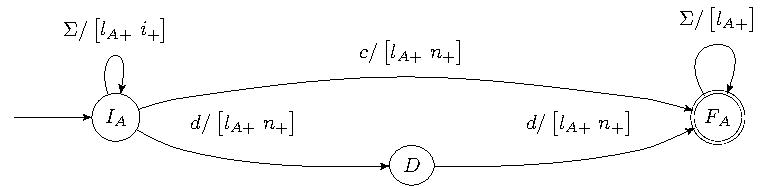
\includegraphics[scale=\autscale]{a}
    \caption{The automaton $A'$, whose Parikh registers count the length of the
    string accepted by the automaton (register $l_A$), the start offset of the
    substring ($i$) and length ($n$) of the substring matching
    $\Regex{c\RegexOr{}dd}$.}\label{fig:aut_a}
      %\Description[SHORT]{LONG}
  \end{subfigure}
  \begin{subfigure}[b]{0.5\textwidth}
    \centering
    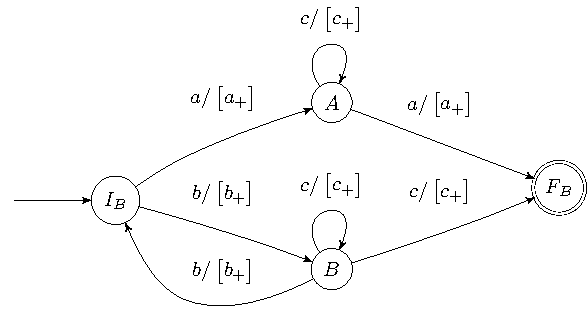
\includegraphics[scale=\autscale]{b}
    \caption{The automaton $B$, where the Parikh registers count the number of
    occurrences of each letter.}\label{fig:aut_b}
      %\Description[SHORT]{LONG}
  \end{subfigure}
  \caption{The collection of automata we use as running
  examples}\label{fig:examples}
\end{figure}


In this section we will introduce an intuition for how a string constraint
problem in an automata-based solver like \OstrichPlus{} is translated to a
Parikh automata intersection problem and solved efficiently using \Calculus{}.
First, by a Parikh automaton we mean a standard non-deterministic finite
automaton (NFA) with a set of Parikh registers that are incremented (or
decremented) at each transition. In the automata of \cref{fig:examples}, we will
use the notation $a / \begin{bmatrix} x_+ \end{bmatrix}$ to mean that a
transition reads an input character $a$ and increments register $x$ by one. We
will omit any zero-valued increments and assume that all registers are scoped to
their automaton. The increments are usually represented as a vector (hence the
notation), but as it is mostly sparse here, we instead use the symbolic notation
$\begin{bmatrix} x_{1+} \end{bmatrix}$ rather than the more cumbersome $\left[
0, 1,  0 , \ldots, 0 \right]$.

Furthermore, we use $\CountOf{c}(A)$ to refer to the number of letters $c$ in
$\Language(A)$, and allow this expression to be used both in linear constraints
of the input language of \cref{ex:string-constraints} and in the langauge of
constraints that we translate to. Where the automaton $A$ is apparent, we will
omit it.

We use standard PCRE regular expressions here and throughout the paper, writing
them $\Regex{\texttt{like this}}$. This means that $\RegexOr{}$ is alternation,
$\mathtt{*}$ the Kleene star, and $\mathtt{.}$, matches any single character.

\begin{example}\label{ex:string-constraints} Consider the following set of
    string constraints:
\begin{constraints}
    \item\label{const:x-in-c-dd} $x \in \Language(\Regex{c\RegexOr{}dd})$.
    \item\label{const:y-in-b} $y \in \Language(B)$, the language accepted by
    automaton~$B$ of \cref{fig:aut_b}.
    \item\label{const:x-substring} $x = \Substring(y, i, n)$, that is $x$ is an
    $n$-length substring of $y$ starting at offset $i$.
    \item\label{const:more-a-than-b} $i = n$, that is the substring is as long as its starting offset.
\end{constraints}
\end{example}

Intuitively, we see that the constraints are satisfiable.
\cref{const:more-a-than-b} implies that the starting offset must be either $1$
or $2$, that is we need to fill out $y$ with either one or two symbols before
the substring $x$ starts. The state $D$ is dead, as $B$ contains no transitions
with label $\Char{d}$, and hence none of the transitions into $D$ can appear in
the intersection of the languages. An example satisfying assignment is $y =
\Char{acca}$, which gives $x = \Char{c}$, $i = 1$, $n = 1$, but others are
possible.

To solve \cref{ex:string-constraints} using \Calculus{},
\cref{const:x-in-c-dd,const:y-in-b,const:x-substring} can be translated to the
product of Parikh automata $B \times A'$, where $A'$ (\cref{fig:aut_a}) is the
Parikh automata obtained by applying the encoding of $\Substring$ described in
\cite{ostrich-plus}. That description can then be used to obtain values for the
subsstring offsets $i, n$. Here follows an intuition for our method on $B \times
A'$ under the global constraint on the substring \cref{const:more-a-than-b}.

Our approach to the computation of the Parikh image (and therefore the solution
to the intersection problem posed by \cref{ex:string-constraints}) consists of
two applications of laziness; late computation of products of automata, and lazy
enforcement of connectivity constraints. Both are in contrast to the eager
approach to finding the Parikh image described in~\cite{generate-parikh-image},
that would have started by computing the product $A' \times B$, translated it to
a Presburger formula with $i, n$ etc as free variables, and then plugged in the
constraint \cref{const:more-a-than-b}.

Starting with an interactive theorem prover and the goal of solving the
constraint $\CountOf{\Char{a}}(B \times A') > \CountOf{\Char{b}}(B \times A')$
we associate each transition of $A'$ and $B$ with a fresh integer variable,
$\TransitionVar_\Transition$, identically to \cite{generate-parikh-image}. These
variables represent how many times each transition is taken. Hence, the final
counter value for each automaton is the element-wise sum:
\begin{equation}
\begin{bmatrix} 
  \CountOf{\Char{a}} \\ \CountOf{\Char{b}} 
  \\ \CountOf{\Char{c}} \\ \CountOf{\Char{d}} 
\end{bmatrix} = \sum_\Transition \TransitionVar_\Transition \cdot 
  \IncrementVec_\Transition \text{ where $\IncrementVec_\Transition$ are the increments of transition $\Transition$}.
\end{equation}

\begin{figure}[h]
    \centering 
  \begin{subfigure}[b]{0.5\textwidth}
    \centering
    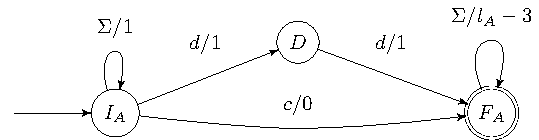
\includegraphics[scale=\autscale]{a_annotated}
    \caption{ $A'$ with its associated transition variables in symbolic form.
    Note: unused ($0$) self-loops at $I_{A'}$ and $F_{A'}$ have been pruned for
    readability.}\label{fig:aut_a_annotated}
      %\Description[SHORT]{LONG}
  \end{subfigure}
  \begin{subfigure}[b]{0.5\textwidth}
    \centering
    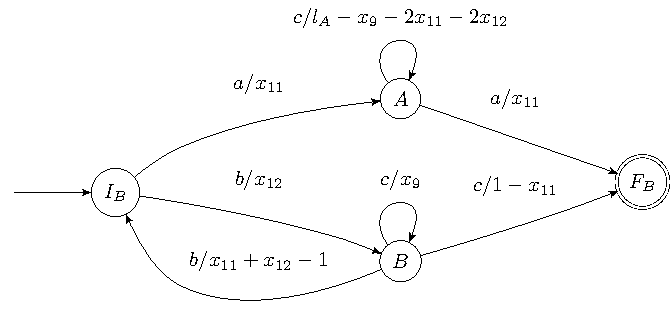
\includegraphics[scale=\autscale]{b_annotated}
    \caption{$B$ with its associated transition variables in symbolic forms.
    Note that state $B$ is now completely dead.}\label{fig:aut_b_annotated}
      %\Description[SHORT]{LONG}
  \end{subfigure}
  \caption{The starting automata, without their counter increments and with
  their transition variables in symbolic form.}\label{fig:propagated}
\end{figure}


We proceed by adding linear constraints requiring transition variables to
represent a flow through either automata by requiring that the number of
incoming transitions is equal to the number of outgoing ones. E.g. state $B$
would have the sum $\cancel{x_{\Tuple{B, \Char{c}, B}}} + x_{\Tuple{I_B,
\Char{b}, B}} = \cancel{x_{\Tuple{B, \Char{c}, B}}}  + x_{\Tuple{B, \Char{c},
F_B}} + x_{\Tuple{B, \Char{b}, I_B}}$ where we let $x_{\Tuple{q, l, c'}}$ refer
to the integer variable associated with a transition from state $q$ to state
$q'$ with label $l$. Note that the self-loop cancels itself out. This means that
for automata where a loop can become unreachable, these constraints do not fully
capture the constraints posed by the automaton, but requires additional
reachability constraints.

Performing symbolic reasoning on these equations and plugging the corresponding
symbolic representation of the constraints on each corresponding integer
variable back as an annotation on its transition, we obtain the two automata in
\cref{fig:propagated}.

% FIXME B-loopen inte nollad här! Uppdatera!

Several transitions are already marked as unuseable (have a transition variable
value of $0$). This includes any transition for the letter $\Char{d}$, as
$\CountOf{\Char{d}}(B) = \sum_{\Transition} 0 = 0$, since the register for
$\Char{d}$ is zero for all transitions in $B$.

Note that the self-loop on state $B$ is nonzero due to the above mentioned
self-balancing. However, a reachability computation will conclude that the state
is unreachable, and allow us to conclude that all its outgoing transitions must
be zero.

After removing all transitions concluded to be unuseable to produce new,
equivalent automata, we compute the product in \cref{fig:product}.

\begin{figure}[h]
    \centering 
    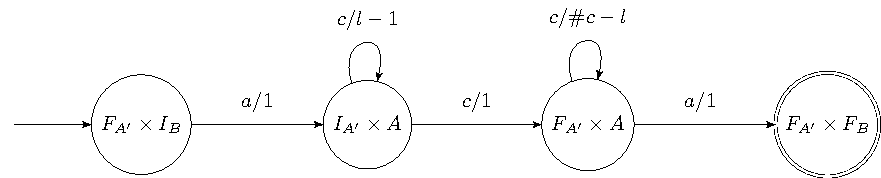
\includegraphics[scale=\autscale]{ab}
  \caption{An automaton encoding the constraint $\CountOf{\Char{a}}(B \times A')
  > \CountOf{\Char{b}}(B \times A')$.}\label{fig:product}
      %\Description[SHORT]{LONG}
\end{figure}

By putting off computing the product $B \times A'$ until after performing linear
reasoning on the number of times each transition must be taken and using that to
prune the terms, we have computed a smaller product than we would have with a
na\"ive approach. Moreover, since this automaton contains only one loop along
one main path, all runs through it can be described by the flow-preservation
equations described above without the need for costly connectivity-enforcing
constraints as in~\cite{generate-parikh-image}. We can now obtain a generalised
solution to our constraints by inspection.